\renewcommand{\FileName}{overview}

\begin{comment}
\begin{frame}[allowframebreaks]
	\frametitle{Categorical Data Analysis: Methods}
Methods of analysis for categorical data fall into two main categories:

\begin{itemize}

\item {\bfseries\large Non-parametric, randomization-based methods}

    \begin{itemize}
    \item make minimal assumptions
    \item useful for hypothesis-testing 
    \item SAS: \PROC{FREQ}; SPSS: Crosstabs
        \begin{itemize*}
        \item Pearson Chi-square
        \item \IX{Fisher's exact test} (for small expected
                frequencies)
        \item Mantel-Haenszel tests (ordered categories: test
                for \emph{linear} association)
        \end{itemize*}
	\item R: \func{chisq.test}, \func{mantelhaen.test}, ...
    \end{itemize}

\framebreak
\item {\bfseries\large Model-based methods}

    \begin{itemize}
    \item Must assume random sample (possibly stratified)
    \item Useful for estimation purposes (std. errors, confidence intervals)
    \item Greater flexibility; fitting specialized models 
		\begin{itemize*}
		 \item Symmetry, quasi-symmetry, structured associations for square tables
		 \item Models for ordinal variables
		\end{itemize*}

    \item More suitable for multi-way tables
    \item SAS: \PROC{LOGISTIC}, \proc{CATMOD}, \proc{GENMOD} , \proc{INSIGHT} (Fit YX)
        \begin{itemize*}
        \item estimate standard errors, covariances for model parameters
        \item confidence intervals for parameters, predicted Pr\{response\}
        \end{itemize*}
    \item R: \func{glm} family, \pkg{car}, \pkg{gnm}, ...
	\item SPSS: Hiloglinear, Loglinear, Generalized linear models
    \end{itemize}

\end{itemize}
\end{frame}
\end{comment}

\begin{frame}
	\frametitle{Categorical data: Analysis methods}
Methods of analysis for categorical data fall into two main categories:

\begin{block}{\large\bfseries Non-parametric, randomization-based methods}
    \begin{itemize}
    \item Make minimal assumptions
    \item Useful for \alert{hypothesis-testing}: Are A and B associated?
    \item Mostly for \alert{two-way} tables (possibly stratified)
    \item SAS: \PROC{FREQ}
        \begin{itemize*}
        \item Pearson Chi-square
        \item \IX{Fisher's exact test} (for small expected frequencies)
        \item Mantel-Haenszel tests (ordered categories: test for \emph{linear} association)
        \end{itemize*}
	\item R: \func{chisq.test}, \func{mantelhaen.test}, ...
	\item SPSS: Crosstabs
    \end{itemize}
\end{block}
\end{frame}

\begin{frame}
	\frametitle{Categorical data: Analysis methods}

\begin{block}{\large\bfseries Model-based methods}
    \begin{itemize}
    \item Must assume random sample (possibly stratified)
    \item Useful for \alert{estimation} purposes: Size of effects (std. errors, confidence intervals)
    \item More suitable for \alert{multi-way} tables
    \item Greater flexibility; fitting specialized models
		\begin{itemize*}
		 \item Symmetry, quasi-symmetry, structured associations for square tables
		 \item Models for ordinal variables
		\end{itemize*}
    \item SAS: \PROC{LOGISTIC}, \proc{CATMOD}, \proc{GENMOD} , \proc{INSIGHT} (Fit YX)
        \begin{itemize*}
        \item estimate standard errors, covariances for model parameters
        \item confidence intervals for parameters, predicted Pr\{response\}
        \end{itemize*}
    \item R: \func{glm} family, \pkg{car}, \pkg{gnm}, ...
	\item SPSS: Hiloglinear, Loglinear, Generalized linear models
    \end{itemize}
\end{block}
\end{frame}

\begin{frame}[label=resp-assoc]
 \frametitle{Categorical data: Response vs. Association models}
  \begin{block}{\large\bfseries Response models}<1->
   \begin{itemize}
    \item Sometimes, one variable is a  natural discrete response.
    \item Q: How does the response relate to explanatory variables?
		\begin{itemize*}
		 \item Admit $\sim$ Gender + Dept
         \item Party $\sim$ Age + Education + Urban
		\end{itemize*}
    \item[$\Rightarrow$] Logit models, logististic regression, generalized linear models
   \end{itemize}
  \end{block}

  \begin{block}{\large\bfseries Association models}<2->
   \begin{itemize}
    \item Sometimes, the main interest is just \alert{association}
    \item Q: Which variables are associated, and \alert{how}?
		\begin{itemize*}
		 \item Berkeley data: [Admit Gender]?  [Admit Dept]? [Gender Dept]
         \item Hair-eye data: [Hair Eye]? [Hair Sex]? [Eye, Sex]
		\end{itemize*}
    \item[$\Rightarrow$] Loglinear models
   \end{itemize}
  \end{block}

   This is similar to the distinction between regression/ANOVA vs.\
   correlation and factor analysis
\end{frame}

\subsection{Graphical methods}
\begin{frame}
  \frametitle{Graphical methods: Tables and Graphs}

  \begin{namedQuote}{Albert Einstein}
  If I can't picture it, I can't understand it.
  \end{namedQuote}
%  \begin{namedQuote}{Yogi Berra}
%  You can see a lot, just by looking.
%  \end{namedQuote}
  \begin{namedQuote}{Farquhar \& Farquhar, 1891}
  Getting information from a table is like extracting sunlight
  from a cucumber.
  \end{namedQuote}


  \begin{block}{\large\bfseries Tables vs.\ Graphs}
      \begin{itemize}
      \item Tables are best suited for \emph{look-up} and calculation---  
		\begin{itemize*}
		 \item read off exact numbers
		 \item additional calculations (e.g., \% change)
		\end{itemize*}

	  \item Graphs are better for:
	  \begin{itemize*}
	      \item showing \emph{patterns, trends, anomalies}, 
	      \item making \emph{comparisons}
	      \item seeing the \emph{unexpected}!
	  \end{itemize*}
	  \item Visual presentation as \emph{communication}: 
	  \begin{itemize*}
			\item what do you want to say or show?
			\item design graphs and tables to 'speak to the eyes'
	  \end{itemize*}
	  \end{itemize}
  \end{block}
\end{frame}


\begin{frame}
\frametitle{Graphical methods: Quantitative data}
Quantitative data (amounts) are  naturally displayed in terms of
	\(
	\mbox{\bf magnitude} \sim \mbox{\bf position along a scale}
	\)

\vspace{1ex}
%% two subfig side-by-side
 \begin{minipage}[t]{.45\textwidth}
  \includegraphics[width=1\linewidth,clip]{fig/lm-income-experience}
  \\ \centering Scatterplot of Income vs. Experience
 \end{minipage}%
 \hfill
 \begin{minipage}[t]{.45\textwidth}
  \includegraphics[width=1\linewidth,clip]{fig/lm-income-gender}
  \\ \centering Boxplot of Income by Gender
 \end{minipage}

\end{frame}

\begin{frame}
\frametitle{Graphical methods: Categorical data}
Frequency data (counts) are more naturally displayed in terms of
	\(
	\mbox{\bf count} \sim \mbox{\bf area}
	\)
	\citep{Friendly:95}

%% two subfig side-by-side
 \begin{minipage}[t]{.45\textwidth}
  \includegraphics[width=1\linewidth,clip]{fig/pie2x2g}
  \\ \centering Fourfold display for 2$\times$2 table
 \end{minipage}%
 \hfill
 \begin{minipage}[t]{.45\textwidth}
  \includegraphics[width=1\linewidth,clip]{fig/mosaic9a3f}
  \\ \centering Mosaic plot for 3-way table
 \end{minipage}

\end{frame}

\begin{frame}

  \begin{itemize}
	\item{\large\bfseries Principles of Graphical Displays}
      \begin{itemize*}
	  \item {\bfseries Effect ordering} \citep{FriendlyKwan:02:effect}--- In tables and graphs, sort unordered factors
	  according to the effects you want to see/show.
	    \vspace{1ex}
		\begin{center}
		\includegraphics[width=.9\textwidth,clip]{fig/corrgram2}
		\end{center}
``Corrgrams: Exploratory displays for correlation matrices'' \citep{Friendly:02:corrgram}
      \end{itemize*}
  \end{itemize}
\end{frame}

\begin{frame}[t]
  \begin{itemize*}
	\item Effect ordering and high-lighting for tables \citep{Friendly:00:mdarray}
%\makeatletter\slidebox@restore\makeatother
	\input{tab/haireye-eff-beamer}
  \end{itemize*}	
\end{frame}

\begin{frame}
  \begin{itemize*}
	  \item {\bfseries Comparisons}--- Make visual comparisons easy
    	\begin{itemize*}
		\item Visual grouping--- connect with lines, make key comparisons contiguous
		\item Baselines--- compare \emph{data} to \emph{model} against a line, preferably horizontal
		\end{itemize*}
  \end{itemize*}
	  \vspace{1ex}
	  \begin{center}
	  \includegraphics[width=.9\textwidth,clip]{fig/madfit2} \\
      \begin{minipage}{.45\linewidth}
      \centering Standard histogram with fit  
      \end{minipage}
		\hfill 
      \begin{minipage}{.45\linewidth}
      \centering Suspended rootogram 
      \end{minipage}
	  \end{center}
\end{frame}

\begin{frame}

  \begin{itemize}
	  \item {\bfseries Small multiples}--- combine stratified graphs into coherent displays \citep{Tufte:83}
    	\begin{itemize*}
		\item e.g., scatterplot matrix for quantitative data: all pairwise scatterplots
		\end{itemize*}
	  \vspace{1ex}
	  \begin{center}
	  \includegraphics[width=.6\textwidth,clip]{fig/prestige22}
	  \end{center}
  \end{itemize}
\end{frame}

\begin{frame}
    \begin{itemize*}
		\item e.g., mosaic matrix for quantitative data: all pairwise mosaic plots
	\end{itemize*}
	  \vspace{1ex}
	  \begin{center}
	  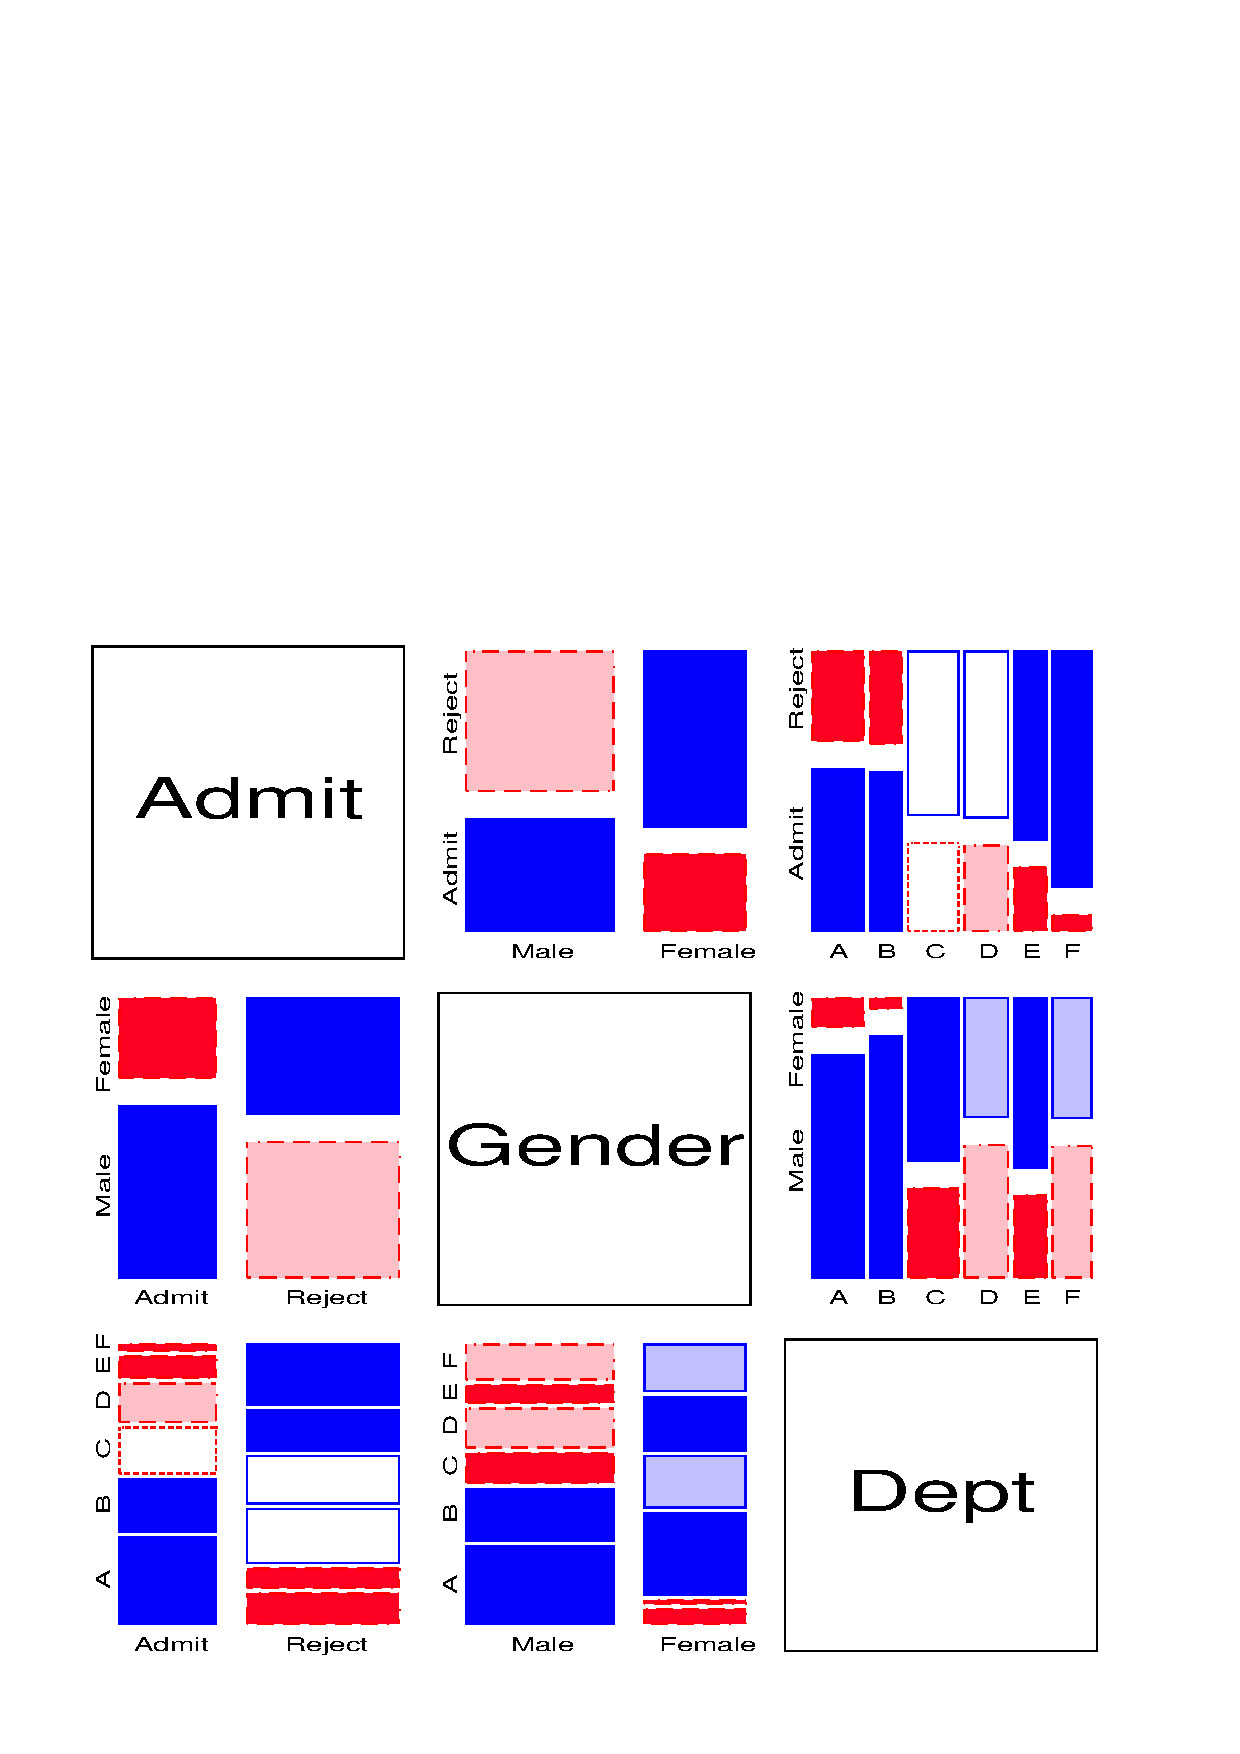
\includegraphics[width=.6\textwidth,clip]{fig/mosmat9a}
	  \end{center}
\end{frame}

\begin{frame}
 \frametitle{Graphical methods: Categorical data}
  \begin{block}{\large\bfseries Exploratory methods}<1->
      \begin{itemize*}
	  \item Minimal assumptions (like non-parametric methods)
	  \item Show the \emph{data}, not just \emph{summaries} 
	  \item Help detect \emph{patterns, trends, anomalies}, suggest hypotheses
	  \end{itemize*}
   \end{block}

	\begin{block}{\large\bfseries Plots for model-based methods}<2->
      \begin{itemize*}
	  \item Residual plots - departures from model, omitted terms, ...
	  \item Effect plots - estimated probabilities of response or log odds 
	  \item Diagnostic plots - influence, violation of assumptions
	  \end{itemize*}
   \end{block}

	\begin{block}{\large\bfseries Goals}<3->
      \begin{itemize*}
	  \item \emph{VCD} and R \pkg{vcd} - Make these methods \emph{available} and \emph{accessible} in SAS \& R
	  \item {\bf Practical power = Statistical power \(\times\) Probability of Use}
	  \item Today's goal:  take-home knowledge
	  \item Tomorrow's goal: dynamic, interactive graphics for categorical data 
	  \end{itemize*}
   \end{block}
\end{frame}

\endinput

% slide template
\begin{frame}
  \frametitle{}
  \begin{itemize}
	\item{\large\bfseries }
      \begin{itemize*}
	  \item 
    	\begin{itemize*}
		\item 
		\item 
		\end{itemize*}
	  \item 
	  \end{itemize*}
	\item{\large\bfseries }
	\item{\large\bfseries }
  \end{itemize}
\end{frame}

